% this TeX file provides an awesome example of how TeX will make super 
% awesome tables, at the cost of your of what happens when you try to make a
% table that is very complicated.
\documentclass[11pt]{article}

% Use wide margins, but not quite so wide as fullpage.sty
\marginparwidth 0.5in 
\oddsidemargin 0.25in 
\evensidemargin 0.25in 
\marginparsep 0.25in
\topmargin 0.25in 
\textwidth 6in \textheight 8 in
% That's about enough definitions

% Line
\newcommand{\HRule}{\rule{\linewidth}{0.5mm}}

% Reference in harvard
%\usepackage[round, authoryear]{natbib}
\usepackage[english]{babel}% Recommended
\usepackage{csquotes}% Recommended

\usepackage[backend=bibtex,
natbib=true,firstinits=true,style=authoryear,sorting=nyt,doi=true,url=true]{biblatex}
\bibliography{references}
\setlength\bibitemsep{1.1\itemsep}

\DeclareNameAlias{sortname}{last-first}

\renewcommand*{\finalnamedelim}{%
  \ifnumgreater{\value{liststop}}{2}{\finalandcomma}{}%
  \addspace\&\space}
  
% pictures!
\usepackage{graphicx}
\graphicspath{ {images/} }

% multirow allows you to combine rows in columns
\usepackage{multirow}
% tabularx allows manual tweaking of column width
\usepackage{tabularx}
% longtable does better format for tables that span pages
\usepackage{longtable}
\usepackage{array}
% counts how many pages there are
\usepackage{lastpage}
%euros
\usepackage{eurosym}
% indent
\usepackage{indentfirst}

% Put bib in TOC
\usepackage[nottoc, section, notlot, notlof]{tocbibind} %nottoc, numbib

% Add H to table to force here
\usepackage{float}
\restylefloat{table}

% maths
\usepackage{amsmath}

% adjust header/footer
\usepackage{fancyhdr}
\pagestyle{fancy}

% URL's
\usepackage{hyperref}
\usepackage{breakurl}

% Appendix
\usepackage[page, titletoc]{appendix}

% Glossery
\usepackage[toc,section=section]{glossaries}
\makeglossaries

% TODO's \todo, \listoftodos, \missingfigure
\usepackage{todonotes}

% Control of footnotes
\usepackage{footmisc}

% header and footer
\rfoot{\thepage\ of \pageref{LastPage}}
\cfoot{}
\lfoot{7565025}

% our document
\begin{document}

\begin{titlepage}
\begin{center}

\textsc{\LARGE University of Manchester}\\[1.5cm]
\textsc{\Large Management, Technology and Innovation Report}\\[0.5cm]

% Title
\HRule \\[0.4cm]
{ \huge \bfseries How does torrenting affect the media industry in the UK? Should the UK continue to block torrenting websites? \\[0.4cm] }

\HRule \\[1.5cm]

% Author and supervisor
\begin{minipage}{0.4\textwidth}
\begin{flushleft} \large
\emph{Author:}\\
Pez \textsc{Cuckow}
\end{flushleft}
\end{minipage}
\begin{minipage}{0.4\textwidth}
\begin{flushright} \large
\emph{Supervisor:} \\
Mohammad \textsc{Hajhashem}
\end{flushright}
\end{minipage}

\vspace{5mm}

\begin{minipage}{0.4\textwidth}
\begin{flushleft} \large
\emph{Student ID:}\\
7565025
\end{flushleft}
\end{minipage}
\begin{minipage}{0.4\textwidth}
\begin{flushright} \large
\emph{Word Count:} \\
1644
\end{flushright}
\end{minipage}

\vspace{5mm}

%TC:ignore
\begin{abstract}
%Torrenting is used to download copyrighted works from the Internet. This report gives an overview of the technology behind it, investigating how it affects the media industry. Evidence is reviewed from global studies to understand its relevance in the legal options accessible in the UK. The negative and opposing effects on the media industry are discussed alongside relevant research data from the UK. The consequence of introducing blocking measures is reviewed from supporting and opposing evidence. In conclusion there are four suggestions for more specific research and legislation related specifically to the  UK media industry.
Torrenting is used to download copyrighted works from the Internet. This report gives an overview of the technology behind it, investigating its effect on the media industry. The consequences of introducing blocking measures is reviewed from supporting and opposing evidence. In conclusion there are four suggestions for more specific research and legislation related specifically to the UK media industry.
\end{abstract}

{\bf Keywords:} BitTorrent, Torrenting, Copyright Law, CDPA
%TC:endignore

\vfill

% Bottom of the page
{\large \today}

\end{center}
\end{titlepage}

% define words
% Glossary
%TC:ignore 
\newglossaryentry{peer}
{
  name=peer,
  description={a user in the BitTorrent network \citep{britannica} }
}

\newglossaryentry{client}
{
  name=client,
  description={a software implementation of the BitTorrent protocol that a peer uses to access the network \citep{britannica} }
}

\newglossaryentry{swarm}
{
  name=swarm,
  description={a group of computers involved in sharing a certain collection of files \citep{swarm} }
}

\newglossaryentry{seeder}
{
  name=seeder,
  description={a user with a fully copy of the files associated with a particular torrent }
}

\newglossaryentry{tracker}
{
  name=tracker,
  description={a server that keeps track of which peers have parts of a particular file and which parts are available for download at a given time. This information is passed to the users client on request, in order to begin downloading the file}
}

\newglossaryentry{isp}
{
  name=ISP,
  description={an Internet service provider (providing access to the Internet for a particular user)  }
}

\newglossaryentry{torrent}
{
  name=torrent,
  description={represents a collection of files, that can be downloaded to a users computer using the BitTorrent protocol \citep{britannica}}
}
%TC:endignore

% the actual contents
% Marking criteria:
%     How good is your question?
%     How well did  answer the question?

% 1500 words + 10% margin
% Do not repeat words: penalties for needless length
% Include name, student number and seminar leaders name
% Produce evidence and support

% Include an abstract (around 50 words)
% Aim at an intelligent reader who does not know about your case
% Make your case interesting and readable

% REPORT
% Use sections (headers and numbers)
% You can use bullet points, graphs, tables, pictures

% Include the research question on the report
% What is the timescale? recent past; future?
% Include the word count

%% _Quantitative_ information is very important achieving a good mark

% Tables/figures/graphs do not go towards the word count
% Page Numbers
% Put graphs inline…

% Figures:
%      Give a figure number and a title
%      Label graphs axes
%      Label units
%      underneath each graph include the reference - detailed source

% Use academic writing style
%     Use third person, don’t use slang, this is a report
%     Use sections/text boxes/bullet points
%
%     Avoid fashionable superlatives

% Don’t do it…
% Very clearly identify quotations with “ “’s and referencing
% To be sure put quotations in italics

% You can use "ideas" but not words…
% Put copied work somewhere else - don’t paste into the original document

% Topics covered
% 1. Introduction: innovation and its pervasive effects; perspectives. 
% 2. Case studies of innovation and impacts. 
% 3. Long term impacts of technological change (Steel processing, computerisation, mass production).
% 4. Economics and technological change. 
% 5. Technology strategy and firms. 
% 6. The role of small firms in innovation. 
% 7. The Product Life Cycle and markets. 
% 8. Networks, standards and formats. 
% 9. Dominant designs, lock-in and systems. 
% 10. Innovation in services. 
% 11. Intellectual property rights: the system and its use. 
% 12. Defence R+D and Innovation.
     
% On your first page include an abstract (very brief description of what the report is about – about 50 words)
% contents list (these are not included abstract)
% Also add a few (3 or 4 or 5?) key words at the end of these are used by journals for indexing

% Example structure
% 1. Introduction
% 2. Development of the Product 500w
% 3. Competition
% 4. Failure in the Market
% 5. Conclusions

\tableofcontents
\listoffigures
\listoftables
\printglossaries

\clearpage

% How does torrenting affect the media industry in the UK?
% Should the UK continue to block torrenting websites?

\section{Introduction} % 100 words

While the technology behind torrenting is legal \citep{MDE:MDE2634}, it is used to download copyrighted materials \citep{currentstateofbittorrent}. %without permission of the publishers 
There is legal controversy over the use of torrent networks \citep{duah2013injunction}. Some users argue the \gls{torrent} network is legal regardless of whether the associated files violate copyright law \citep{piratebaylegal}.

Piracy has been a concern for the media industry since the `double deck' cassette player allowed users to duplicate cassettes. In the digital age, media can be duplicated and distributed on torrent networks. \citep{cameron2014audio, currentstateofbittorrent}.

This report will highlight how the increase of copyrighted works being `torrented' affects the UK media industry and will review the effectiveness of the UK torrent blocks.

\section{Torrenting} %400 words

`Torrenting' is slang referring to the downloading of files using the BitTorrent protocol \citep{britannica}, a popular \Gls{peer} to Peer (P2P) file-sharing network\footnote{Further details in Appendix \ref{app:bittorrent}} \citep{p2pmeasurements, cachelogictruep2p, cachelogicp2p2}. 
%  that has ``stood the test of time''

\subsection{Popularity}

\citet{sandvinereport} found that BitTorrent was the most popular P2P protocol in Europe, second only to YouTube in overall Internet traffic (Table~\ref{table:sandvinereport}).

Moving from the growth phase to the maturity stage of the product lifecycle, access to BitTorrent is becoming easier due to enhanced torrent \glspl{client}, better understanding, and easy to follow tutorials. It is at the early majority stage in the technology adoption lifecycle with conservative users beginning to use the network. 

% Table 6 - Top 10 Peak Period Applications - Europe, Fixed Access
\begin{table}[h]
\centering
\begin{tabular}{llllllll}
           & \multicolumn{2}{c}{Uploads}                          & \multicolumn{2}{c}{Downloads}         & \multicolumn{2}{c}{Aggregate}                 &        \\
Rank       & Application                       & Share            & Application         & Share            & Application         & Share            &        \\
\hline
\textbf{1} & \textbf{BitTorrent}               & \textbf{48.10\%} & YouTube             & 28.73\%          & YouTube             & 24.21\%          &        \\
2          & YouTube                           & 7.12\%           & HTTP                & 15.64\%          & \textbf{BitTorrent} & \textbf{17.99\%} &        \\
3          & HTTP                              & 5.74\%           & \textbf{BitTorrent} & \textbf{10.10\%} & HTTP                & 13.59\%          &        \\
4          & Skype                             & 4.96\%           & Facebook            & 4.94\%           & Facebook            & 4.65\%           &        \\
5          & Facebook                          & 3.54\%           & Netflix             & 3.45\%           & Netflix             & 3.33\%           &        \\
6          & Netflix                           & 2.83\%           & MPEG - Other        & 3.10\%           & MPEG - Other        & 2.57\%           &        \\
7          & SSL                               & 2.47\%           & RTMP                & 2.82\%           & RTMP                & 2.42\%           &        \\
8        & eDonkey                  & 1.12\%  & Flash Video         & 2.56\%           & Skype               & 2.32\%           &        \\
9          & Dropbox                           & 1.12\%           & SSL                 & 1.91\%           & Flash Video            & 2.16\% \\
10         & RTMP                              & 0.85\%           & PutLocker           & 1.25\%           & SSL                 & 2.03\%           &        \\
           & \multicolumn{1}{r}{Total Tracked} & 77.83\%          &                     & 73.23\%          &                     & 75.25\%          &       
\end{tabular}
\caption{Top 10 Peak Period Applications, Europe \citep{sandvinereport}}
\label{table:sandvinereport}
\end{table}

\subsection{Technology}

It is important to differentiate between a `traditional download' and one on the BitTorrent network. Traditionally, a remote server stores the file which downloads to the user \citep[Chapter 7.]{reese2000java}.
%
On the BitTorrent network, the file is downloaded from the other network users whilst simultaneously uploading `pieces' of the file to one another \citep{bittorrentrobustness2003} (Fig.~\ref{fig:clientVSp2p}).
% 
This process starts with a \textit{.torrent}\footnote{Downloaded from the selected tracker} which contains important information but significantly no part of the file itself\footnote{Appendix \ref{app:torrentprocess}} \citep{bittorrentrobustness2003}. 


\begin{figure}[h]
    \centering
    \includegraphics[width=0.8\textwidth]{clientvsp2p}
    \caption{Client/Server VS Peer2Peer Network \citep{gogrid}}
    \label{fig:clientVSp2p}
\end{figure}

The network operates on an incentive basis; each user's download speed is scaled by a sharing ratio (Fig~\ref{figure:scaling}), discouraging users from sharing slows the network and reduces the files available \citep{bittorrentrobustness2003}.

\begin{figure}[h]
    \centering
    
    \[ \mbox{share ratio} = \frac{\mbox{total data uploaded}}{\mbox{total data downloaded}} \]
    
    \caption{Share/seeding ratio equation for a BitTorrent client \citep{bittorrentrobustness2003}}
    \label{figure:scaling}
\end{figure}

\section{Intellectual Property Rights}

% SHOULD I DEFINE COPYRIGHT AS AN EXAMPLE OF IPR?
As BitTorrent operates without a central authority, liability for copyright infringement on the network falls upon the users of the system \citep{currentstateofbittorrent}.

\subsection{Legal Options}
There are two legal options for firms wishing to discourage torrenting of their content; place liability on those who are sharing the content (uploading) or on those who are downloading content.
%
However it is technically difficult\footnote{See Appendix \ref{app:legaloptions} for further details.} to track a download occurring \citep{MDE:MDE2634}.

% Move to the appendix?
As knowledge of how to effectively prosecute has increased \citep{currentstateofbittorrent}, prosecutors are no longer targeting the individual users, but the \glspl{tracker} supporting the network, such as The Pirate Bay \citep[p.179 - 181]{fungvsmpaa, intellectualproperty}.

\subsection{In the UK}

Most trackers are based abroad \citep{top10trackers2014}, meaning responsibility of prosecution falls within international intellectual property law \citep[III.]{currentstateofbittorrent}.
%
To avoid this complexity, UK media companies, represented by the British Phonographic Industry (BPI)\footnote{More than 300 music and record companies in the UK \citep{bpi2013}}, sought to make the \gls{isp}'s providing access to the copyrighted content liable \citep{bpivsukisps, meale2013triple}.

% What is an ISP?
The landmark case was BPI vs. The 6 Largest UK \gls{isp}'s\footnote{Who held a ``fixed line market share of 94\% of Internet users in the UK'' at the time}. The court concluded\footnote{See Appendix \ref{app:bpiVtpb}} that both the users and the operators of The Pirate Bay were liable for copyright infringement.
%
The final judgement served an injunction against the \gls{isp}'s as ``service providers'' \citep[97A]{cdpa} ordering them to `adopt technical means to block'' access to The Pirate Bay\footnote{In addition to any website designed to enable access} \citep{bpivsukisps, meale2013triple}.

The number of blocks against UK \gls{torrent} websites has increased since 2012, with relevant judgements referring to this case. In 2013, 28 websites\footnote{See Table~\ref{table:courtorders} in the appendix.} were found guilty of file sharing and blocked \citep{emivsisp, footballvseztv, skycopyright, bbcblock21, bbcblocks2, meale2013premier}.

\subsection[Keeping IP Laws Up to Date]{Keeping Intellectual Property Laws Up to Date}

% "In 2010 it was claimed that implementation of blocks would generate a 70% reduction in online copyright infringement (using file sharing)." \lse{2013}

To address online copyright infringement, the Digital Economy Act (DEA) was written. There are two phases; 1. sending warnings to customers suspected of infringement;
%If this is unsuccessful in decreasing copyright infringement, 
2. allowing ISP's to disconnect persistent infringers from the Internet \citep{dea2010}.

There is strong opposition against the act. \citet{lse2011} found that it ``gets the balance between copyright enforcement and innovation wrong''. They highlighted \textit{disruptive technologies}, such as the Photocopier and Cassette Recorder, previously blamed by the media industry for loss of revenue. % however industry innovation has accommodated them into modern life.
% The research suggests that instead of enforcing ``heavy-handed'' copyright law
Research suggests the music industry should focus on enabling ``users to download music legally at a reasonable price'' \citep{lse2011}.
%
It was also found that the decline in sales of recorded music could be attributed to other factors, including changing music consumption patterns, decreasing disposable income, and increasing sales of digital content (see Fig.~\ref{fig:digitalrevenue}).

\begin{figure}[h]
    \centering
    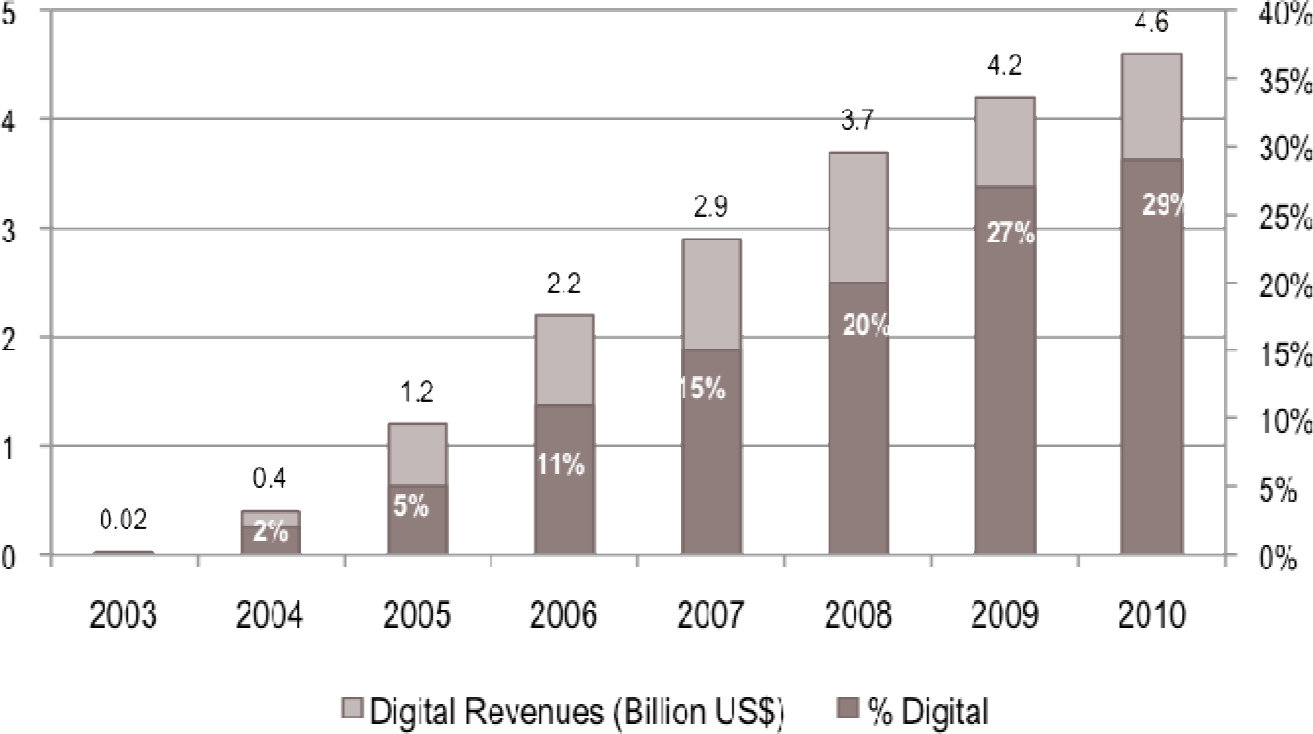
\includegraphics[width=0.8\textwidth]{digitalrevenue}
    \caption{Worldwide online sales of music 2004-2010. Adapted from \citet[Fig. 3]{lse2011}}
    \label{fig:digitalrevenue}
\end{figure}

% What is the infrincement
% Suing the downloaders
% Suing the uploders
% Going after the trackers

\section{Effect of Torrenting}

\citet{pwc2009} reports that there was a decline in recorded and digital music sales across the EU from 2004 to 2008, with revenues in the digital market falling by 26\%. Research until 2011 (Fig~\ref{fig:musicindustry}) shows this decline continuing. Further studies attribute this decrease to digital piracy \citep{tera2010,peitz2004,zentner2006}. The UK media industry supports this conclusion \citep{factuk2014, ccc2014, bpi2013}.

\begin{figure}[h]
    \centering
    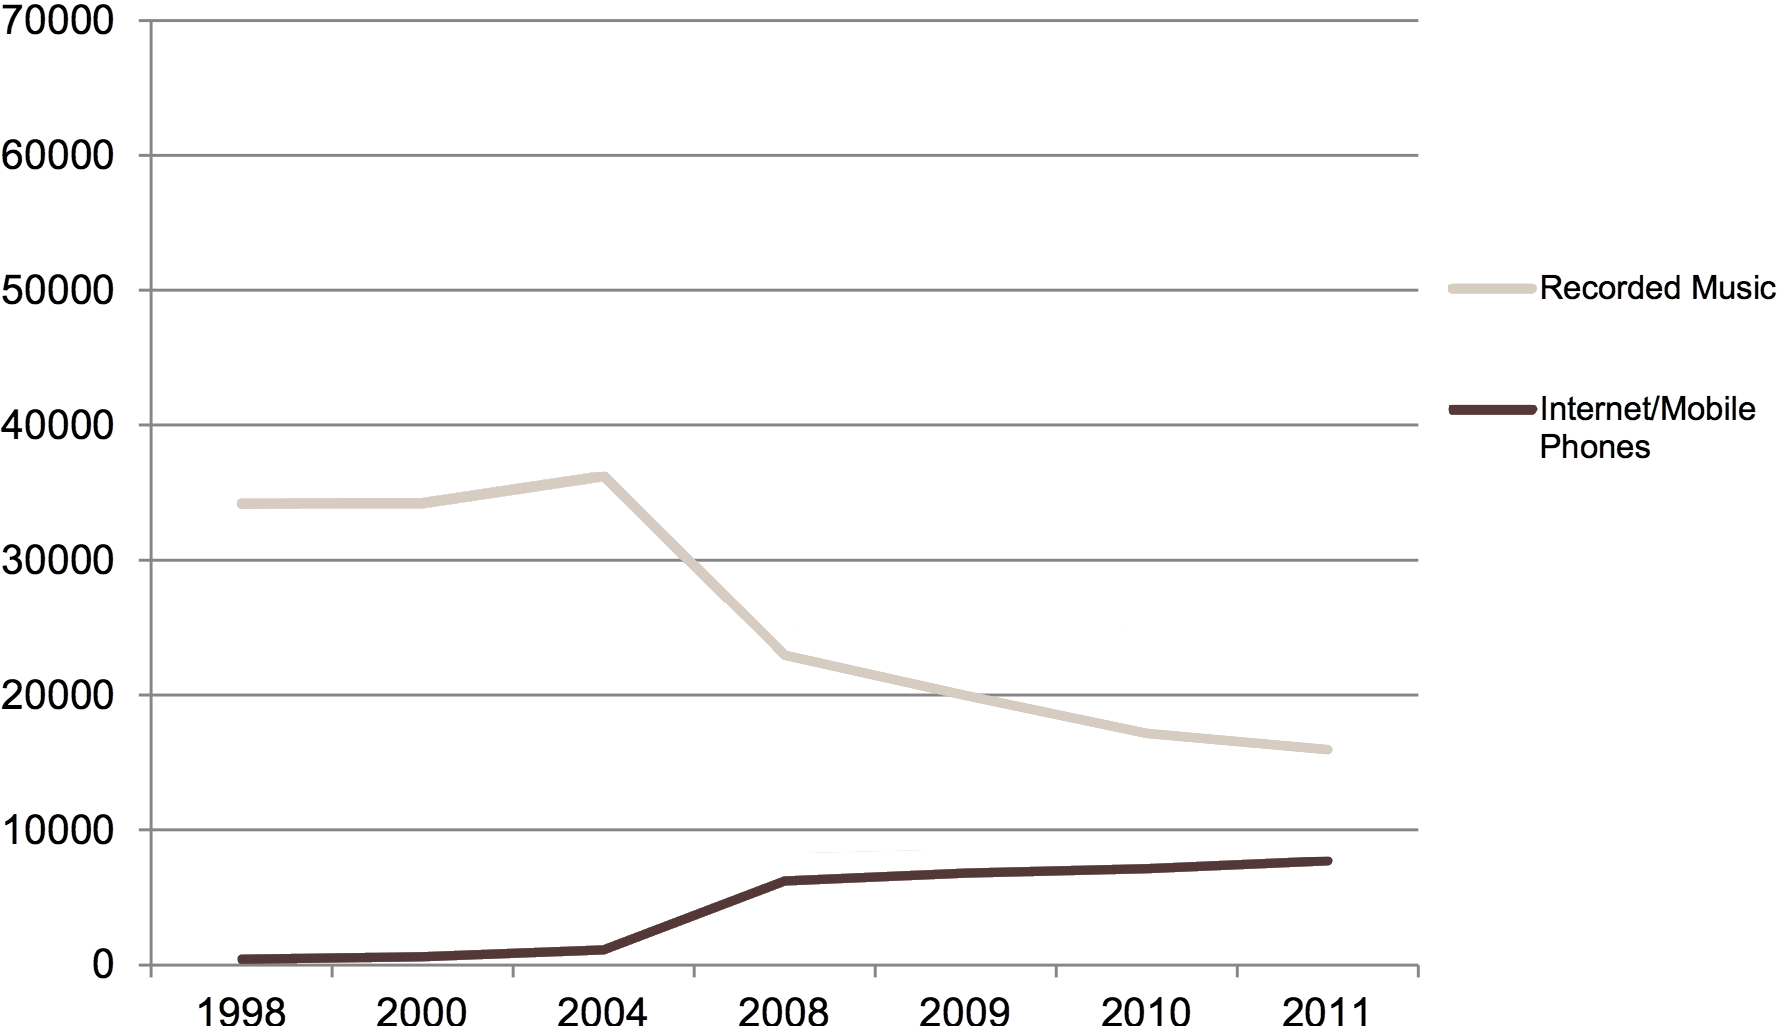
\includegraphics[width=0.8\textwidth]{musicindustry}
    \caption{Trends in Revenues of the Music Industry, USD Million. Adapted from \citet[Fig. 1]{lse2013}}
    \label{fig:musicindustry}
\end{figure}

%On the other hand
Conversely, research from the London School of Economics suggests torrenting might increase revenue in the media industry \citep{lse2013, hammond13,aguiar2013}.

\subsection{Negative Effects}

The International Chamber of Commerce commissioned a report\footnote{As part of the Business Action to Stop Counterfeiting and Piracy (BASCAP) initiative} quantifying the effects of ``piracy on retail revenue'' \citep{tera2010}.  
%
%The research split the creative industries into `core'\footnote{``Press and literature'' and ``Music, Video, Software''} and `non-core'\footnote{Any industry that supports the former, such as manufacturers of televisions or musical instruments}.
Using data from the European Commission Eurostat database \citep{eurostat}, \citet{tera2010} calculated the value of the UK ``creative industries'' (Table~\ref{table:creativeindustryweight}), finding the creative industries form 6.2\% of UK GDP. %, and employ 5.4\% of the UK workforce.
%
%Taking the number of infringements per year (Table~\ref{table:infringementsperyear}) and applying a substitution rate (see Table~\ref{table:substitution}) 
The loss to the media industry\footnote{Calculated taking the number of infringements per year (Table~\ref{table:infringementsperyear}), applying a substitution rate (Table~\ref{table:substitution})} in 2008 was \pounds{533} million\footnote{\label{foot1}Figures converted from EUR to GBP at 0.796651, the average 2008 exchange rate \citep{exchangerate2008}.}\footnote{Loss to music was \pounds{224} million, film \pounds{245} million and TV series \pounds{62} million.} \citep[p.31]{tera2010}.

\begin{table}[h]
\centering
\begin{tabular}{lll}
                              & Value Added & Number of Employees \\
\hline
Core                          & 6.2\%       & 5.4\% \\
Interdependent \& support     & 3.4\%       & 3.8\% \\
TOTAL creative industries     & 9.6\%       & 9.2\% \\
GDP (billion \euro)           & 175         &       \\
Employment (million)          &             & 2.7   \\
\end{tabular}
\caption{Weight of Creative Industries in the UK \citep[Table 5]{tera2010}}
\label{table:creativeindustryweight}
\end{table}
\begin{table}[h]
\centering
\begin{tabular}{ll}
Media     & Copyright infringements per year (M unit) \\ \hline
Music     & 1,177                                \\
Film      & 98.05                                \\
TV Series & 53.33                               
\end{tabular}

\caption{Digital piracy in the United Kingdom \citep{tera2010}}
\label{table:infringementsperyear}
\end{table}
\begin{table}[h]
\centering
\begin{tabular}{ll}
Media (Position on Release Timeline)            & Substitution Rate \\
\hline
Music (Released) & 10\%   \\
Film (Cinema)   & 5\% \\
Film (DVD)      & 10\% \\
Film (TV)      & 10\% \\
TV Series (TV)  & 30\% \\
TV Series (DVD) & 5\% \\
TV Series (PayPerView) & 2\%
\end{tabular}
\caption{Substitution rate, representing percentage of units likely sold if piracy was eliminated \citep[p.19, Table 6]{tera2010}}
\label{table:substitution}
\end{table}


% recorded music context, we have based our assumptions on a conservative 10%


The report concludes that piracy significantly harms the creative industries and as broadband becomes more commonplace, without ``sustained and effective action'' \citep[p.46]{tera2010}, digital piracy in Europe will continue to grow, in line with similar reports \citep{europeeconomics2008, oecd2009}. As these reports are often commissioned by bodies representing the media industry their reliability is questionable.

\subsection{Opposition}

Research by \citet{lse2013} extends findings from \citet{lse2011}, that ``data provided by the music industry were misleading'' and the ``industry was doing reasonably well.''. It concludes that the evidence reviewed did not support the claims from the media industry of `revenue reduction' due to copyright infringement.
% Make this shorter
They found ``punitive measures'' in France proposed by the industry did not have the desired impact, with the HAPOPI'\footnote{An acronym of the department that the law created} law being abolished\footnote{See Appendix \ref{app:hadopi}}.

\citet{lse2013} recommend that the DEA needs to be reviewed, following independent research, to form fair legislation on copyright infringement.
%\citet{lse2013} recommends, following independent research of the media industries claims that the DEA needs to be reviewed, to form fair legislation on copyright infringement.

A report by \citet{aguiar2013}\footnote{commissioned by the European Joint Research Centre,}, observed the digital media purchasing patterns of 16,000 European consumers, finding increases in illegal downloads and legal streaming led to an increase in legal purchases, with a \textit{purchase elasticity} of 0.04 and a \textit{`visit' elasticity} 0.06.

%Finding the  was positive and linear at 0.04 , noting that a 10\% increase in illegal downloading lead to a 0.2\% increase in legal purchases.
%In addition they found that a 10\% increase in visits to legal streaming websites lead to a 0.7\% , with an elasticity of 0.06 in the UK, supporting the innovation in the media industry would lead to increases in media sales.

Further research from \citet{hammond13} looked into the effect of media `leaked'\footnote{Download available from BitTorrent before the official release} onto BitTorrent, finding that leaked albums cause a small increase in legal sales and not the decrease the media industry claims.
%``small relative to ... promotional efforts'' such as plays on the radio. 
% LORNA SAYS DELETE THIS

\section{Blocks in the UK}

The UK media industry has been successful in securing High Court injunctions against \glspl{isp}'s, ordering them to ``adopt ... technical means'' \citep{bpivsukisps} to block trackers supporting BitTorrent network, with the intention of cutting copyright infringement. 

New evidence suggests that blocks have been ineffective in reducing torrenting, however the findings should be taken lightly due to the recent nature of the reports, limited supporting evidence, and lack of peer reviews \citep{bbc2012piratebay, duah2013injunction}. % and that they're not research papers

%%%%% OTHERS NEEDED HERE %%%%

\subsection{Supporting Evidence}

When discussing the effectiveness of previous blocks, the \citet{bpivsukisps} noted that blocking the Pirate Bay in Italy had resulted in a 73\% reduction in visits and a 96\% reduction of page views \citep{meale2013triple}.

The \citet{ndpgroup2013} cited in \citet{ribeiro2013court} noted a decline in illegal music sharing on P2P during 2012, observing a 17\% decrease in activity, but added that ``The primary reason for the reduced sharing ... was an increased use of free, legal music streaming services'' and not the blocks put in place.

Despite being cited in news articles defending the blocks \citep{bbc2012piratebay}, the BPI and others from the media industry are yet to reference any evidence demonstrating their effectiveness in reducing UK activity on BitTorrent.

\subsection{Opposing Evidence}

In a University of Westminster debate, Google's UK policy manager Theo Bertram opposed the blocks, highlighting that targeting the business is more effective, referring to the ``now-defunct'' MegaUpload\footnote{A popular file hosting service, commonly used for piracy},  explaining that its supply has ``shifted to ... middle-ranking pirate sites.''. He warned that targeting individual piracy sites ends in a game of ``whac-a-mole'' \citep{torrentfreak2013google, musictank2013}.

\citet{bbc2012piratebay} reported one week after the block of the Pirate Bay, falling ``illegal download traffic'' on one \gls{isp}'s network returned to normal as users found ways around the blocks.
%
It is easy for both the operators of trackers and the users to circumvent them\footnote{Particularly with the haste of services designed to avoid the block}\footnote{Appendix \ref{app:avoidingblocks}} \citep{duah2013injunction, bbc2012piratebay, proxylist2014, comein2014}.
%
The BPI defended the block, noting statistics (Fig. \ref{fig:piratebayblock}) from Nielsen Net Ratings showing traffic to the Pirate Bay website had dropped \citep{bbc2012piratebay}.

\begin{figure}[h]
    \centering
    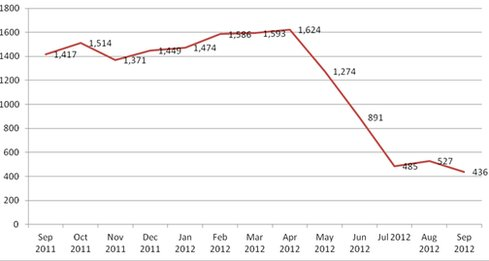
\includegraphics{piratebayblock}
    \caption{Traffic to The Pirate Bay (\citet{nielsen2012} cited in \citet{bbc2012piratebay})}
    \label{fig:piratebayblock}
\end{figure}

The Open Rights Group\footnote{Who campaign on digital rights and freedom issues \citep{org2014}} responded to the blocks, stating that blocking is extreme and will lead to ``new forms of distributed infringement''. They advised the BPI's tactics ``may have the opposite effect'', ``legitimising and promoting resistance to their actions.'' \citep{killock2013ORG}.
%adding ``users and the public interest have not been represented in the processes'' .

\citet{duah2013injunction} discusses the blocks, commenting they do not offer a ``complete solution'' and that a ``significant number of blocks'' is needed to effectively cover all infringing websites.
%
Enforcing a block is not a passive process, as the copyright holder or the \gls{isp} must continually scan the situation to keep the blocks up to date. \citet{duah2013injunction} notes it is still unclear who is responsible for this task.

\section{Conclusions}

% "It is quite unusual to include references in this section, as it is mainly a review of what has already been said."

Given the position of BitTorrent in the product and technology adoption lifecycles, usage will continue to increase and as such, clear evidence based legislation is needed.

The case against BitTorrent references reports commissioned by the UK media industry increasing the likelihood of bias. Independent reports argue in favour of BitTorrent, suggesting other factors, including changing music consumption patterns and increasing sales of digital content, affect the media industry.

Initial research suggests the use of blocks to control access to copyright material is ineffective and that blocks are easy to mitigate. It has yet to be shown that blocks lead to any decrease in the activity of sharing on the BitTorrent network.

Having reviewed the evidence:
\begin{enumerate}
\item Independent research into the effect of digital piracy on the media industry needs to be completed to offer a more reliable base for decisions.
\item The effect of the recent tracker blocks on sharing copyrighted material on the BitTorrent network in the UK should be researched.
\item On completion of this further research, the DEA should be revised in light of the findings to support the legislation or suggest changes.
\item The media industry should innovate legal uses of BitTorrent to distribute media and drive sales, rather than continuing to pursue legal means to prevent its use. %, as seen with driving sales of music using radio.
\end{enumerate}
 
Overall, to justify continuing to block torrenting websites, significant independent evidence that the blocks are effective, and that torrenting is negatively affecting the media industry, is needed. 

In future, when updating UK law, the government should observe research from independent sources, rather than from those whom the law may benefit.

Finally, the media industry may benefit from adopting BitTorrent, working with this technology, rather than against it.


% references

%\addcontentsline{toc}{chapter}{References}
%\bibliographystyle{plainnat}
\printbibliography
% printbibliography[<options for printing>]

% appendix
%TC:ignore
\setcounter{table}{0}
\renewcommand{\thetable}{A\arabic{table}}

\begin{appendices}

\section{BitTorrent} \label{app:bittorrent}

Created by Bram Cohen and formalised in 2008, BitTorrent supports P2P filesharing and is commonly used to distribute large files over the Internet with the individual peers, rather than a single server bearing the load and costs \citep{cohen2008} . 

\subsection{Popularity}
Since 2004, BitTorrent has been the most popular P2P protocol (holding 53\% of total P2P traffic) with other competing  protocols such as FastTrack, Gnutella and eDonkey falling in both users and traffic \citep{cachelogictruep2p, cachelogicp2p2}.

\subsection{Overview} \label{app:torrentprocess}

On BitTorrent, users downloading the file are leechers and once the file is complete, seeders, uploading the file to other users in the network. \Glspl{peer} with a particular file are called the `swarm'. Fig.~\ref{fig:architecture} shows an overview of the BitTorrent network during a download.

\begin{figure}[h]
    \centering
    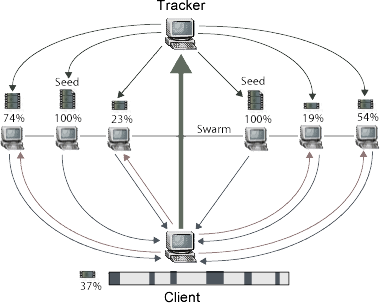
\includegraphics[width=0.6\textwidth]{architecture}
    \caption{Architecture of the BitTorrent network  \citet{history13}}
    \label{fig:architecture}
\end{figure}

\section{Prosecuting a User} \label{app:legaloptions}

\citet{MDE:MDE2634} argues that the usual intent of lawsuits against torrenters is to ``change user behaviour'' in an attempt to discourage users from sharing files on the network and not to recover ``meaningful damages''. ``Discouraging users'' has been key since Chan Nai-ming, the first person to be convicted of piracy, who was sentenced to 3 months imprisonment \citep{bigcrook07}.

In order to prosecute an individual user of the BitTorrent network, the prosecution must present evidence of that user using the network to download or share copyrighted works without permission of the copyright holder.

\subsection{Downloading}
It is difficult to track a download occurring due to the distributed nature of the P2P network.
Pieces of the file come from many different locations at once, no one server provides the whole file so it's hard to link the connections to one instance of infringement. Additionally, because the file is split into many pieces, it is problematic to prove each piece is a part of a copyrighted work. Legally, even if a download is witnessed it must be proven that the downloader is deliberately infringing copyright.

\subsection{Sharing}
Demonstrating sharing is technically simple. A user would simply need to request a particular \textit{.torrent} from the \gls{swarm} and log those listed as peers who have copies of the file available for download. This would also serve as a legal demonstration of the intent to distribute copyright-protected material.

\section{Prosecuting a Tracker}
There have been several successful, high profile cases against the \glspl{tracker} that index the copyrighted works to make them available to the general downloader \citep{fungvsmpaa}.
Commonly in the United Kingdom, the legal responsibility now falls against the Internet Service Provider's (\gls{isp}'s)  that provide access to the \glspl{tracker}, rather than the \glspl{tracker} themselves \citep{bpivsukisps}. Due to the multinational nature of the Internet, there is often complication as to with whom jurisdiction falls.

\section{BPI vs UK ISP's} \label{app:bpiVtpb}

Dramatico Entertainment Limited, Emi Records Limited, Mercury Records Limited, Polydor Limited, Rough Trade Records Limited,Sony Music Entertainment UK Limited, Virgin Records Limited, Warner Music Uk Limited, and 679 Recordings Limited vs. British Sky Broadcasting Limited, British Telecommunications Plc, Everything Everywhere Limited, Talktalk Telecom Group Plc, Telefonica UK Limited, and Virgin Media Limited.

\subsection{Charges}
The court found the users guilty on two counts. Firstly, copying as defined in section 17 of the Copyright, Designs and Patents Act (CDPA) \citep{cdpa}; arguing that by selecting a torrent, a user is willing infringing copyright and highlighting that during download the file contents are copied to the user's computer. Secondly, ``communicating to the public'' as defined in section 20 of CDPA, citing  ``communication to the public must be interpreted broadly'' (\citet[47.]{courtofjustice2012} as cited in \citet{bpivsukisps}) in order to apply it to the Internet and that ``at least 15\% of the sample records were being shared'' \citep{bpivsukisps}.

The court found the operators of The Pirate Bay guilty of authorisation or assisting the infringement; pointing out that the operators go far beyond enabling and assisting the copyright infringement, 
 they ``sanction, approve and countenance'' and that they are ``providing means to infringe, encouraging infringement and taking no steps to prevent'' it \citep{bpivsukisps}.

\section{HADOPI} \label{app:hadopi}

In an attempt to limit the spread of piracy throughout France, the French government created a dedicated department agency, the High Authority for Transmission of Creative Works and Copyright Protection on the Interne, to address this problem and to increase sales in the French media industry.
This department was mandated to identify and prosecute French Internet users who had been identified as sharing or downloading copyrighted materials using a three strike system, starting with education and ending in prosecution, disconnection from the Internet and fine's.
However, after enforcing this law and sending out over a million warnings, research found that increased sales stemmed from the education component of the `HADOPI law' \citep{danaher2012hadopi}, and not the prosecution element as expected. This suggested that prosecution of copyright infringers did not deter people from digital piracy \citep{peoples2012hadopi}. 

In May 2013 a government report recommended the removal of the law \citep{lescure2013}. In July 2013 the French government abolished the law choosing to target `commercial piracy' and `sites that profit from pirated material' \citet{guardian2013hadopi}.

\section{Avoiding the Blocks} \label{app:avoidingblocks}

It is easy to avoid blocks, anybody could do it following a tutorial, particularly with the rapid increase of tutorials and proxies following a block. For example simply typing `pirate bay proxy' into Google returns hundreds of websites designed to avoid the blocks.

The operators can also perform one of many tricks to mitigate the blocks due to the technical way that the blocks are enforced, including change of a servers IP address and use of a different domain \citep{piratebaylegal}.

\section{Tables}

\begin{table}[H]
\centering
\begin{tabular}{m{2cm}m{3cm}m{7cm}m{2cm}}
\textbf{By} & \textbf{Against} & \textbf{Reason} & \textbf{Date} \\
\hline
BPI &   The Pirate Bay            & Authorisation of copyright infringement & May 2012 \\
FACT-UK & \begin{tabular}[l]{@{}l@{}}Fenopy\\ H33t\\ KickassTorrents\end{tabular}                                                                                & Enabling mass access to infringing content        & March 2013  \\
MPAA & Movie2k                  & \textit{Court order not published}        & May 2013  \\
MPAA & Download For All         & \textit{Court order not published}        & May 2013  \\
FACT-UK \& MPAA & EZTV          & Communication to the public (of copyrighted content)       & July 2013 \\
PPL \& BPI & \begin{tabular}[l]{@{}l@{}}
1337x\\
Abmp3\\
Bit Snoop\\
BeeMPS\\
Bomb-Mp3e\\ 
Mp3World\\ 
ExtraTorrent\\ 
File Crop\\ 
FilesTube\\ 
Monova\\ Mp3 Juices\\ Mp3lemon\\ Mp3 Raid\\ Mp3 Skull\\ New Album Releases\\ Rapid Library\\ Torrent Crazy\\ Torrent Downloads\\ Torrent Hound\\ Torrent Reactor\\ Torrentz
\end{tabular}                   & Commercially exploiting music without a licence & October 2013  \\
FACT-UK & YIFY Torrents                   & Communication to the public (of copyrighted content) & November 2013 \\
\end{tabular}

\caption{UK Court ordered blocks against file sharing websites \citep{emivsisp, footballvseztv, skycopyright, bbcblock21, bbcblocks2}}
\label{table:courtorders}
\end{table}

\end{appendices}
%TC:endignore




\end{document}
